\documentclass[tikz]{standalone}
\usepackage{physics}
\usepackage{amsmath}
\usepackage{tikz}
\usepackage{mathdots}
\usepackage{yhmath}
\usepackage{cancel}
\usepackage{color}
\usepackage{siunitx}
\usepackage{array}
\usepackage{multirow}
\usepackage{amssymb}
\usepackage{gensymb}
\usepackage{tabularx}
\usepackage{extarrows}
\usepackage{booktabs}
\usetikzlibrary{fadings}
\usetikzlibrary{patterns}
\usetikzlibrary{shadows.blur}
\usetikzlibrary{shapes}
\begin{document}



\tikzset{every picture/.style={line width=0.75pt}} %set default line width to 0.75pt        

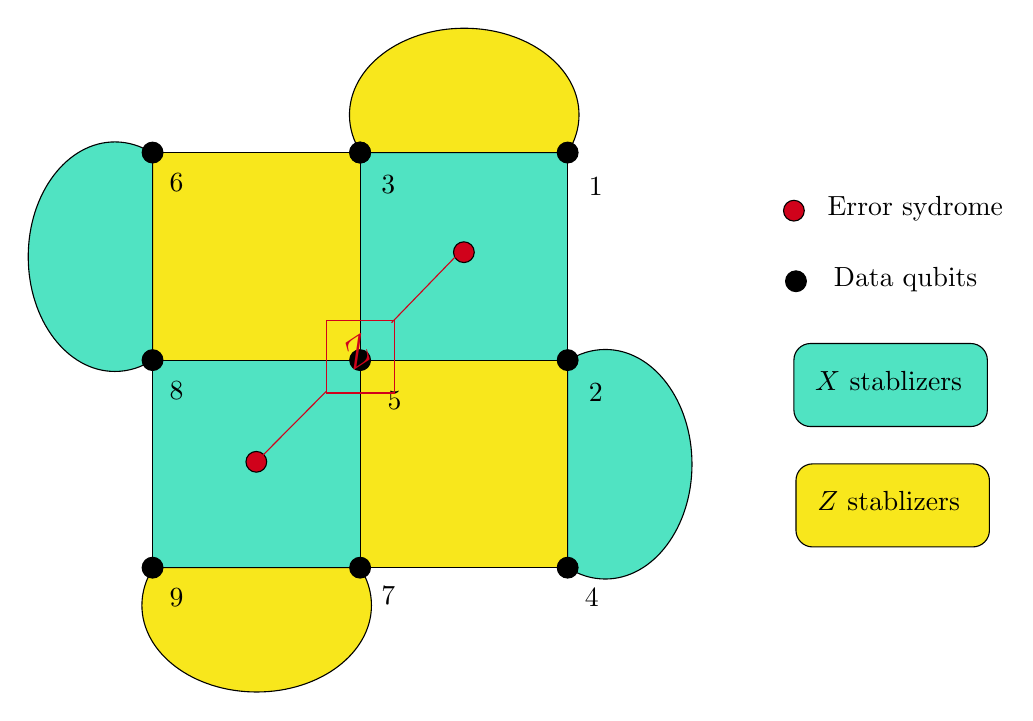
\begin{tikzpicture}[x=0.75pt,y=0.75pt,yscale=-1,xscale=1]
%uncomment if require: \path (0,380); %set diagram left start at 0, and has height of 380

%Shape: Grid [id:dp48727269628607006] 
\draw  [draw opacity=0][fill={rgb, 255:red, 80; green, 227; blue, 194 }  ,fill opacity=1 ] (109,74) -- (309,74) -- (309,274) -- (109,274) -- cycle ; \draw   (209,74) -- (209,274) ; \draw   (109,174) -- (309,174) ; \draw   (109,74) -- (309,74) -- (309,274) -- (109,274) -- cycle ;
%Shape: Grid [id:dp2267510879985528] 
\draw  [draw opacity=0][fill={rgb, 255:red, 248; green, 231; blue, 28 }  ,fill opacity=1 ] (109,74) -- (209,74) -- (209,174) -- (109,174) -- cycle ; \draw    ; \draw    ; \draw   (109,74) -- (209,74) -- (209,174) -- (109,174) -- cycle ;
%Shape: Grid [id:dp38817050469639025] 
\draw  [draw opacity=0][fill={rgb, 255:red, 248; green, 231; blue, 28 }  ,fill opacity=1 ] (209,174) -- (309,174) -- (309,274) -- (209,274) -- cycle ; \draw    ; \draw    ; \draw   (209,174) -- (309,174) -- (309,274) -- (209,274) -- cycle ;
%Shape: Chord [id:dp17082868329548073] 
\draw  [fill={rgb, 255:red, 80; green, 227; blue, 194 }  ,fill opacity=1 ] (109,174) .. controls (103.51,177.51) and (97.36,179.47) .. (90.86,179.47) .. controls (67.8,179.47) and (49.1,154.71) .. (49.1,124.17) .. controls (49.1,93.63) and (67.8,68.87) .. (90.86,68.87) .. controls (97.36,68.87) and (103.51,70.83) .. (109,74.34) -- cycle ;
%Shape: Chord [id:dp4145300199009935] 
\draw  [fill={rgb, 255:red, 248; green, 231; blue, 28 }  ,fill opacity=1 ] (209.34,74) .. controls (205.83,68.51) and (203.87,62.36) .. (203.87,55.86) .. controls (203.87,32.8) and (228.63,14.1) .. (259.17,14.1) .. controls (289.71,14.1) and (314.47,32.8) .. (314.47,55.86) .. controls (314.47,62.36) and (312.51,68.51) .. (309,74) -- cycle ;
%Shape: Chord [id:dp1386005192975044] 
\draw  [fill={rgb, 255:red, 80; green, 227; blue, 194 }  ,fill opacity=1 ] (309,174.34) .. controls (314.49,170.83) and (320.64,168.87) .. (327.14,168.87) .. controls (350.2,168.87) and (368.9,193.63) .. (368.9,224.17) .. controls (368.9,254.71) and (350.2,279.47) .. (327.14,279.47) .. controls (320.64,279.47) and (314.49,277.51) .. (309,274) -- cycle ;
%Shape: Chord [id:dp6513490035985291] 
\draw  [fill={rgb, 255:red, 248; green, 231; blue, 28 }  ,fill opacity=1 ] (209,274) .. controls (212.51,279.49) and (214.47,285.64) .. (214.47,292.14) .. controls (214.47,315.2) and (189.71,333.9) .. (159.17,333.9) .. controls (128.63,333.9) and (103.87,315.2) .. (103.87,292.14) .. controls (103.87,285.64) and (105.83,279.49) .. (109.34,274) -- cycle ;
%Shape: Circle [id:dp12063745964738704] 
\draw  [fill={rgb, 255:red, 0; green, 0; blue, 0 }  ,fill opacity=1 ] (104,74) .. controls (104,71.24) and (106.24,69) .. (109,69) .. controls (111.76,69) and (114,71.24) .. (114,74) .. controls (114,76.76) and (111.76,79) .. (109,79) .. controls (106.24,79) and (104,76.76) .. (104,74) -- cycle ;
%Shape: Circle [id:dp9166888193581574] 
\draw  [fill={rgb, 255:red, 0; green, 0; blue, 0 }  ,fill opacity=1 ] (304,74) .. controls (304,71.24) and (306.24,69) .. (309,69) .. controls (311.76,69) and (314,71.24) .. (314,74) .. controls (314,76.76) and (311.76,79) .. (309,79) .. controls (306.24,79) and (304,76.76) .. (304,74) -- cycle ;
%Shape: Circle [id:dp2932087421862295] 
\draw  [fill={rgb, 255:red, 0; green, 0; blue, 0 }  ,fill opacity=1 ] (204,74) .. controls (204,71.24) and (206.24,69) .. (209,69) .. controls (211.76,69) and (214,71.24) .. (214,74) .. controls (214,76.76) and (211.76,79) .. (209,79) .. controls (206.24,79) and (204,76.76) .. (204,74) -- cycle ;
%Shape: Circle [id:dp1925383620698462] 
\draw  [fill={rgb, 255:red, 0; green, 0; blue, 0 }  ,fill opacity=1 ] (204,74) .. controls (204,71.24) and (206.24,69) .. (209,69) .. controls (211.76,69) and (214,71.24) .. (214,74) .. controls (214,76.76) and (211.76,79) .. (209,79) .. controls (206.24,79) and (204,76.76) .. (204,74) -- cycle ;
%Shape: Circle [id:dp38595673795197005] 
\draw  [fill={rgb, 255:red, 0; green, 0; blue, 0 }  ,fill opacity=1 ] (104,174) .. controls (104,171.24) and (106.24,169) .. (109,169) .. controls (111.76,169) and (114,171.24) .. (114,174) .. controls (114,176.76) and (111.76,179) .. (109,179) .. controls (106.24,179) and (104,176.76) .. (104,174) -- cycle ;
%Shape: Circle [id:dp6253883372750996] 
\draw  [fill={rgb, 255:red, 0; green, 0; blue, 0 }  ,fill opacity=1 ] (304,174) .. controls (304,171.24) and (306.24,169) .. (309,169) .. controls (311.76,169) and (314,171.24) .. (314,174) .. controls (314,176.76) and (311.76,179) .. (309,179) .. controls (306.24,179) and (304,176.76) .. (304,174) -- cycle ;
%Shape: Circle [id:dp45783528141465224] 
\draw  [fill={rgb, 255:red, 0; green, 0; blue, 0 }  ,fill opacity=1 ] (204,174) .. controls (204,171.24) and (206.24,169) .. (209,169) .. controls (211.76,169) and (214,171.24) .. (214,174) .. controls (214,176.76) and (211.76,179) .. (209,179) .. controls (206.24,179) and (204,176.76) .. (204,174) -- cycle ;

%Shape: Circle [id:dp47452567951997804] 
\draw  [fill={rgb, 255:red, 0; green, 0; blue, 0 }  ,fill opacity=1 ] (104,274) .. controls (104,271.24) and (106.24,269) .. (109,269) .. controls (111.76,269) and (114,271.24) .. (114,274) .. controls (114,276.76) and (111.76,279) .. (109,279) .. controls (106.24,279) and (104,276.76) .. (104,274) -- cycle ;
%Shape: Circle [id:dp16037869673699567] 
\draw  [fill={rgb, 255:red, 0; green, 0; blue, 0 }  ,fill opacity=1 ] (304,274) .. controls (304,271.24) and (306.24,269) .. (309,269) .. controls (311.76,269) and (314,271.24) .. (314,274) .. controls (314,276.76) and (311.76,279) .. (309,279) .. controls (306.24,279) and (304,276.76) .. (304,274) -- cycle ;
%Shape: Circle [id:dp6008000754972171] 
\draw  [fill={rgb, 255:red, 0; green, 0; blue, 0 }  ,fill opacity=1 ] (204,274) .. controls (204,271.24) and (206.24,269) .. (209,269) .. controls (211.76,269) and (214,271.24) .. (214,274) .. controls (214,276.76) and (211.76,279) .. (209,279) .. controls (206.24,279) and (204,276.76) .. (204,274) -- cycle ;

%Shape: Circle [id:dp2334944165307784] 
\draw  [fill={rgb, 255:red, 208; green, 2; blue, 27 }  ,fill opacity=1 ] (254,122) .. controls (254,119.24) and (256.24,117) .. (259,117) .. controls (261.76,117) and (264,119.24) .. (264,122) .. controls (264,124.76) and (261.76,127) .. (259,127) .. controls (256.24,127) and (254,124.76) .. (254,122) -- cycle ;
%Shape: Circle [id:dp14453838947025155] 
\draw  [fill={rgb, 255:red, 208; green, 2; blue, 27 }  ,fill opacity=1 ] (154,223) .. controls (154,220.24) and (156.24,218) .. (159,218) .. controls (161.76,218) and (164,220.24) .. (164,223) .. controls (164,225.76) and (161.76,228) .. (159,228) .. controls (156.24,228) and (154,225.76) .. (154,223) -- cycle ;
%Straight Lines [id:da8669723952041025] 
\draw [color={rgb, 255:red, 208; green, 2; blue, 27 }  ,draw opacity=1 ]   (192.8,188.95) -- (159,223) ;
%Straight Lines [id:da2545513005747483] 
\draw [color={rgb, 255:red, 208; green, 2; blue, 27 }  ,draw opacity=1 ]   (258,121) -- (224.16,155.96) ;
%Rounded Rect [id:dp5217908904951286] 
\draw  [fill={rgb, 255:red, 80; green, 227; blue, 194 }  ,fill opacity=1 ] (418,174) .. controls (418,169.58) and (421.58,166) .. (426,166) -- (503.2,166) .. controls (507.62,166) and (511.2,169.58) .. (511.2,174) -- (511.2,198) .. controls (511.2,202.42) and (507.62,206) .. (503.2,206) -- (426,206) .. controls (421.58,206) and (418,202.42) .. (418,198) -- cycle ;
%Shape: Circle [id:dp05560876107531043] 
\draw  [fill={rgb, 255:red, 0; green, 0; blue, 0 }  ,fill opacity=1 ] (414,136) .. controls (414,133.24) and (416.24,131) .. (419,131) .. controls (421.76,131) and (424,133.24) .. (424,136) .. controls (424,138.76) and (421.76,141) .. (419,141) .. controls (416.24,141) and (414,138.76) .. (414,136) -- cycle ;
%Rounded Rect [id:dp21843878551076623] 
\draw  [fill={rgb, 255:red, 248; green, 231; blue, 28 }  ,fill opacity=1 ] (419,232) .. controls (419,227.58) and (422.58,224) .. (427,224) -- (504.2,224) .. controls (508.62,224) and (512.2,227.58) .. (512.2,232) -- (512.2,256) .. controls (512.2,260.42) and (508.62,264) .. (504.2,264) -- (427,264) .. controls (422.58,264) and (419,260.42) .. (419,256) -- cycle ;
%Shape: Circle [id:dp43150251856527233] 
\draw  [fill={rgb, 255:red, 208; green, 2; blue, 27 }  ,fill opacity=1 ] (413,102) .. controls (413,99.24) and (415.24,97) .. (418,97) .. controls (420.76,97) and (423,99.24) .. (423,102) .. controls (423,104.76) and (420.76,107) .. (418,107) .. controls (415.24,107) and (413,104.76) .. (413,102) -- cycle ;

% Text Node
\draw (318,85) node [anchor=north west][inner sep=0.75pt]  [font=\normalsize] [align=left] {{\fontfamily{helvet}\selectfont 1}};
% Text Node
\draw (318,184) node [anchor=north west][inner sep=0.75pt]  [font=\normalsize] [align=left] {{\fontfamily{helvet}\selectfont 2}};
% Text Node
\draw (218,84) node [anchor=north west][inner sep=0.75pt]  [font=\normalsize] [align=left] {{\fontfamily{helvet}\selectfont 3}};
% Text Node
\draw (316,283) node [anchor=north west][inner sep=0.75pt]  [font=\normalsize] [align=left] {{\fontfamily{helvet}\selectfont 4}};
% Text Node
\draw (221,188) node [anchor=north west][inner sep=0.75pt]  [font=\normalsize] [align=left] {{\fontfamily{helvet}\selectfont 5}};
% Text Node
\draw (116,83) node [anchor=north west][inner sep=0.75pt]  [font=\normalsize] [align=left] {{\fontfamily{helvet}\selectfont 6}};
% Text Node
\draw (218,282) node [anchor=north west][inner sep=0.75pt]  [font=\normalsize] [align=left] {{\fontfamily{helvet}\selectfont 7}};
% Text Node
\draw (116,183) node [anchor=north west][inner sep=0.75pt]  [font=\normalsize] [align=left] {{\fontfamily{helvet}\selectfont 8}};
% Text Node
\draw (116,283) node [anchor=north west][inner sep=0.75pt]  [font=\normalsize] [align=left] {{\fontfamily{helvet}\selectfont 9}};
% Text Node
\draw  [color={rgb, 255:red, 208; green, 2; blue, 27 }  ,draw opacity=1 ]  (192.66,155.05) -- (225.4,155.05) -- (225.4,189.82) -- (192.66,189.82) -- cycle  ;
\draw (196.59,168.02) node [anchor=north west][inner sep=0.75pt]  [font=\Large,color={rgb, 255:red, 208; green, 2; blue, 27 }  ,opacity=1 ,rotate=-326.84]  {$Z$};
% Text Node
\draw (436,128) node [anchor=north west][inner sep=0.75pt]   [align=left] {Data qubits};
% Text Node
\draw (427,178) node [anchor=north west][inner sep=0.75pt]   [align=left] {$\displaystyle X$ stablizers};
% Text Node
\draw (428,236) node [anchor=north west][inner sep=0.75pt]   [align=left] {$\displaystyle Z$ stablizers};
% Text Node
\draw (433,94) node [anchor=north west][inner sep=0.75pt]   [align=left] {Error sydrome};


\end{tikzpicture}
\end{document}